\chapter{Perancangan Database}

\section{Perancangan Power Designer}
Setelah menganalisis proses bisnis dan dokumen yang diperlukan, maka selanjutnya kita membuat design diagram di power designer. Pada tahap ini kita harus bisa menganalisis Relasi antar Entity, Kardinalitas sebuah relasi, dan Mandatory relasi. Hal pertama yang harus dilakukan yaitu membuat conceptual data model-nya. berikut gambar design yang telah kami buat.\\

\begin{figure}[H]
	\centering
	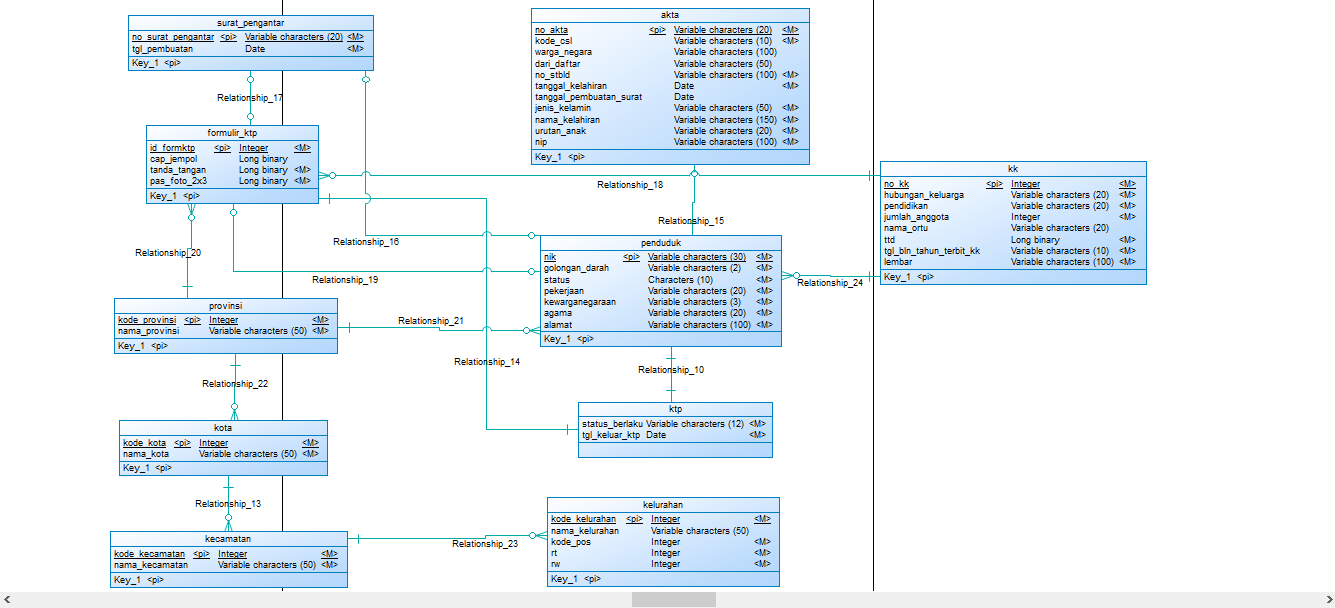
\includegraphics[width=20cm]{figures/cdm.png}
	\caption{Conceptual Data Model.}	
\end{figure}

berdasarkan analisis proses bisnis dan dokumen yang kami lakukan, kami menyimpulkan ada 10 entity yang harus dibuat. Pada masing-masing entity kami menganalisis lagi berdasarkan atribut yang ada pada entity, atribut yang cocok untuk dijadikan primary key seperti yang terlihat pada gambar diatas, setelah membuat entity dan menentukan primary key, selanjutnya kita buat relasi. Dalam membuat relasi kita harus menentukan terlebih dahulu derajat kardinalitasnya, apakah hubungan antar tabel tersebut satu ke satu, satu ke banyak, banyak ke satu, atau banyak ke banyak. Setelah itu, tentukan mandatory relasi tersebut, apakah mandatory atau tidak. Hubungan relasi proses pembuatan ktp :
\begin{enumerate}
\item Relasi antara tabel kelurahan dengan tabel kecamatan (many-one)
Satu kecamatan memiliki satu atau banyak kelurahan dan setiap kelurahan harus memiliki satu dan hanya satu kecamatan\\
\item Relasi antara tabel kecamatan dengan tabel kota (many-one)
Satu kota memiliki satu atau banyak kecamatan dan setiap kecamatan harus memiliki satu dan hanya satu kota.\\
\item Relasi antara tabel kota dengan tabel provinsi (many-one)
Satu provinsi memiliki satu atau banyak kota dan setiap kota harus memiliki satu dan hanya satu provinsi.\\
\item Relasi antara tabel formulir dengan tabel provinsi (one-one)
satu formulir harus memiliki satu dan hanya satu provinsi dan satu provinsi harus memiliki satu dan hanya satu formulir. \\
\item Relasi antara tabel penduduk dengan tabel provinsi (one-many)
Satu penduduk memiliki satu dan hanya satu provinsi dan setiap provinsi memiliki satu atau banyak penduduk. \\
\item Relasi antara tabel penduduk dengan tabel kartu keluarga (one-many)
Satu penduduk harus memiliki satu dan hanya satu kartu keluarga dan setiap kartu keluarga memiliki satu atau lebih penduduk.\\
\item Relasi antara tabel penduduk dengan tabel ktp (one-one)
Satu penduduk harus memiliki satu dan hanya satu ktp dan setiap ktp harus memiliki satu dan hanya satu penduduk\\
\item Relasi antara tabel penduduk dengan tabel akta (one-one)
Satu penduduk harus memiliki satu dan hanya satu akta dan setiap akta harus memiliki satu dan hanya satu penduduk\\
\item Relasi antara tabel penduduk dengan tabel surat pengantar (one-one)
Satu penduduk memiliki satu dan hanya satu surat pengantar dan setiap surat pengantar harus memiliki satu dan hanya satu penduduk\\
\item Relasi antara tabel penduduk dengan tabel formulir (one-one)
Satu penduduk memiliki satu dan hanya satu formulir dan setiap formulir harus memiliki satu dan hanya satu penduduk\\
\item Relasi antara tabel surat pengantar dengan tabel formulir (one-many)
Satu surat pengantar memiliki satu dan hanya satu formulir dan setiap formulir harus memiliki satu dan hanya satu penduduk\\
\end{enumerate}

